\documentclass[a4paper, norsk, 10pt]{article}
\usepackage[utf8]{inputenc} % Vise norske tegn
%\usepackage[T1]{fontenc} 
\usepackage{multicol, fancyhdr}
\usepackage[norsk, english]{babel} % Tilpasning til norsk
\usepackage[margin=2cm]{geometry}
\usepackage{graphicx}
\usepackage{wrapfig}
%\usepackage{array, xcolor}
%\definecolor{ligttgray}{gray}{0.8}
\usepackage[mmddyyyy]{datetime}
\usepackage[table]{xcolor}
\usepackage{fancyhdr} %For å lage topptekst og bunntekst
\newcommand\tab[1][1cm]{\hspace*{#1}}
\pagestyle{fancy}
\fancyhead[R]{Notat om skjemaer}

\title{\bfseries \huge Skjemaer og annen brukerinput \\ Informasjonsteknologi 2, 2017/18}
\date{}
\author{}

\begin{document}
\thispagestyle{fancy}
\maketitle

\section*{Informasjon}
Notatet beskriver fire ulike måter å ta inn brukerverdier på dersom man ikke ønsker å bruke prompt:
\begin{enumerate}
\item Tekstbokser
\item Avkrysningsbokser
\item Radioknapper
\item Knapper
\end{enumerate} 
\ \\
Disse har ulike  bruksområder, der dere selv må ta en vurdering på hva som egner seg til bruk når. Legg merke til at jeg ikke trenger å bruke $<$form$>$ når jeg skal styre innholdet med javascript. Her presenteres syntax for og eksempler på de fire, både hvordan man skal legge dem til og hvordan man skal bruke inputen videre.\\
\ \\
\clearpage
\section*{HTML}
\begin{tabular}{|p{10cm}|p{6cm}|}
\hline
\multicolumn{2}{|c|}{\large{Tekstbokser (text, number) } \cellcolor{lightgray}} \\
$<$input type="text"  id="tekstinput"$>$ &$\bullet$ taggen \textit{placeholder = tekst} gir en tekst i feltet frem til det skrives inn noe \\
$<$input type="number"  id="tallinput"$>$& $\bullet$ \textit{type="number"} brukes når inputen er tall \\
\multicolumn{2}{|c|}{\large{Avkrysningsbokser  (checkbox) } \cellcolor{lightgray}} \\
$<$input type="checkbox" name="checkinput" value="valg1" id="checkinput1"$>$ Valg 1 & $\bullet$ legg inn linjeskift etter hver input\\
\multicolumn{2}{|c|}{\large{Radioknapper (radio) } \cellcolor{lightgray}} \\
$<$input type="radio" name="radioinput" id="radioinput1"$>$ Valg 1 & $\bullet$ legg inn linjeskift etter hver input \\
\multicolumn{2}{|c|}{\large{Knapper (button)} \cellcolor{lightgray}} \\
$<$button id="knapp"$>$ Tekst som vises $<$/button$>$& \\
\hline
\end{tabular}
\begin{figure}[h!]
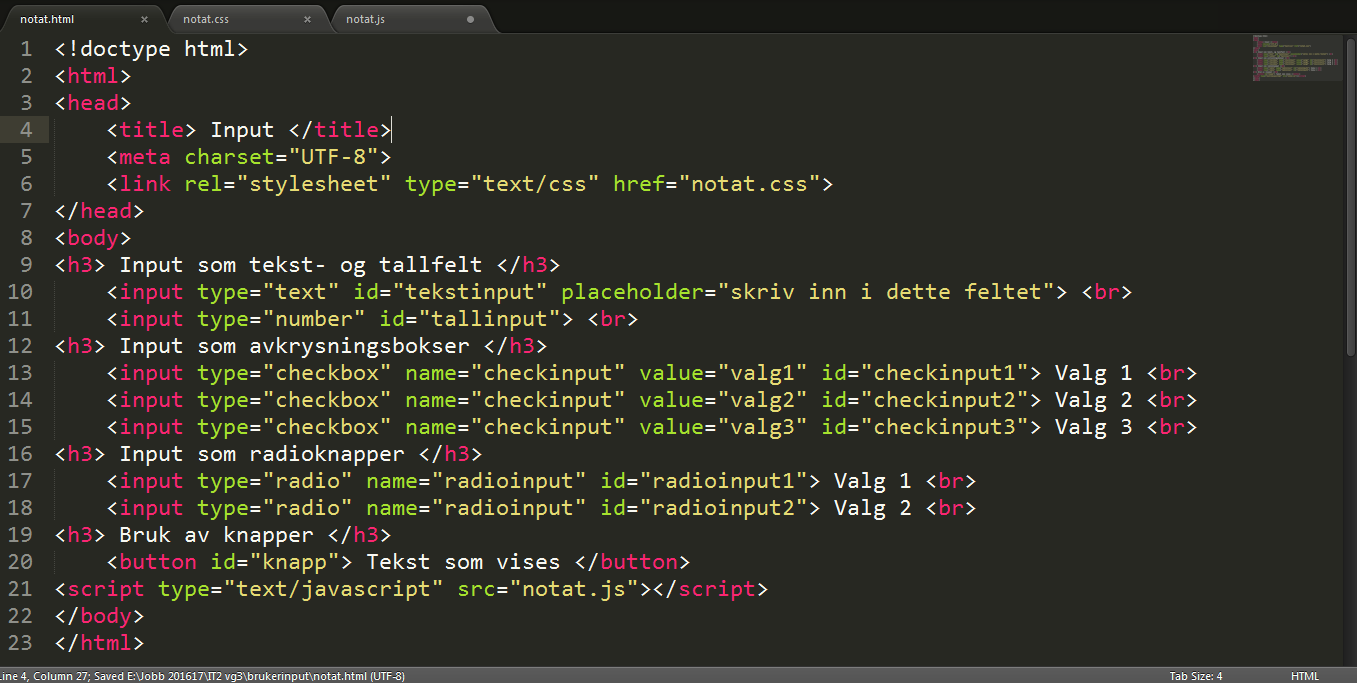
\includegraphics[width=0.8\linewidth]{html1.png}
\end{figure}
\begin{figure}[h!]
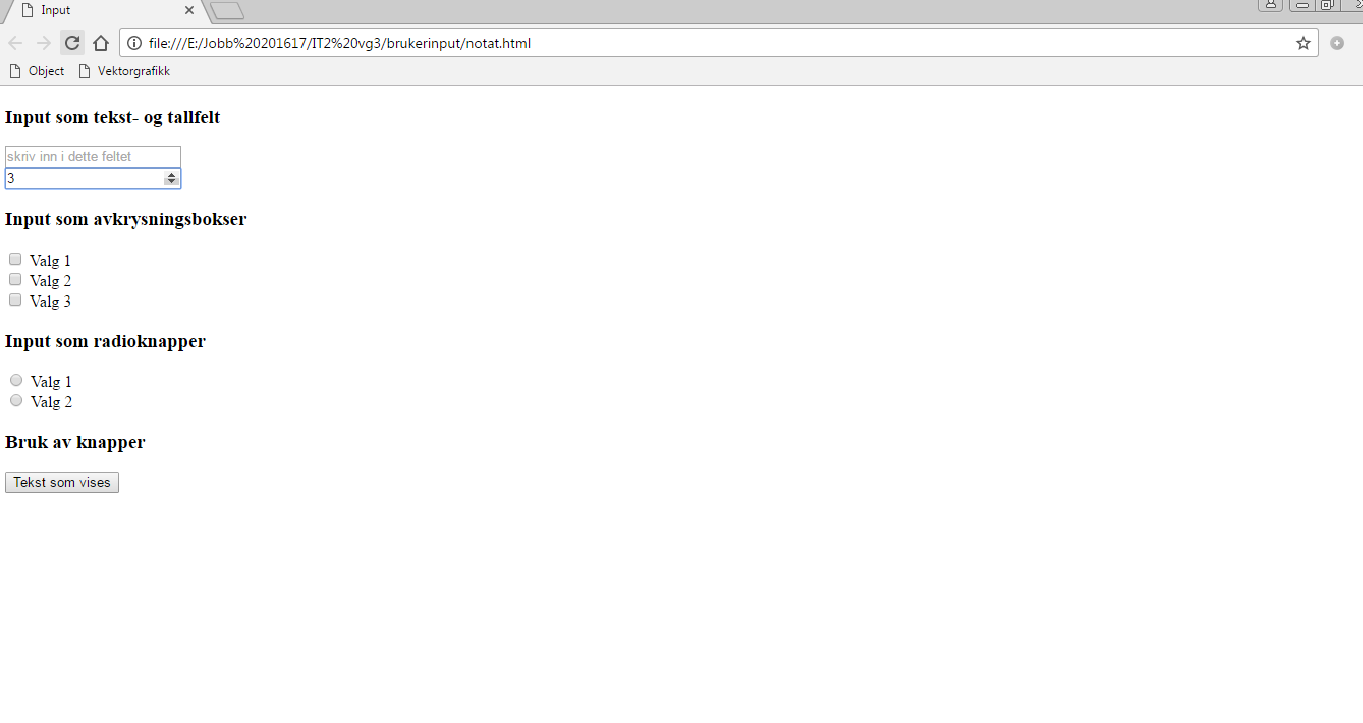
\includegraphics[width=0.8\linewidth]{html2.png}
\end{figure}

\clearpage
\section*{CSS}
\begin{tabular}{|p{10cm}|p{6cm}|}
\hline
\multicolumn{2}{|c|}{\large{Tekstbokser (text, number) } \cellcolor{lightgray}} \\
input$[$type="text"$]$,$[$type="number"$]\{$ & $\bullet$ kan spesifisere str på boksen \\
\tab width:50$\%$; & eller skriften, som vanlig\\
$\}$ & $\bullet$ kan også referere direkte til idene\\
\multicolumn{2}{|c|}{\large{Avkrysningsbokser (checkbox) og radioknapper (radio) } \cellcolor{lightgray}} \\
input$[$type="checkbox"$]$, $[$type="radio"$]\{$ & $\bullet$ ellers lite å stilsette  her \\
\tab cursor: pointer;& $\bullet$ kan også referere direkte til idene\\
$\}$& \\
input:checked$\{$& \\
\tab height: 20px;& \\
\tab width: 20px;& \\
$\}$& \\
\multicolumn{2}{|c|}{\large{Knapper (button)} \cellcolor{lightgray}} \\
button$\{$ & $\bullet$ her er dett mange muligheter, \\
\tab background-color: $\#$f2f2f2; & se på knappen som en boks \\
\tab color:  $\#$323232;& og legg til border og padding som vanlig \\
\tab cursor: pointer;&\\
$\}$ &\\
button:active$\{$&\\
\tab color:  $\#$CC0000;&\\
$\}$&\\
\hline
\end{tabular}
\begin{figure}[h!]
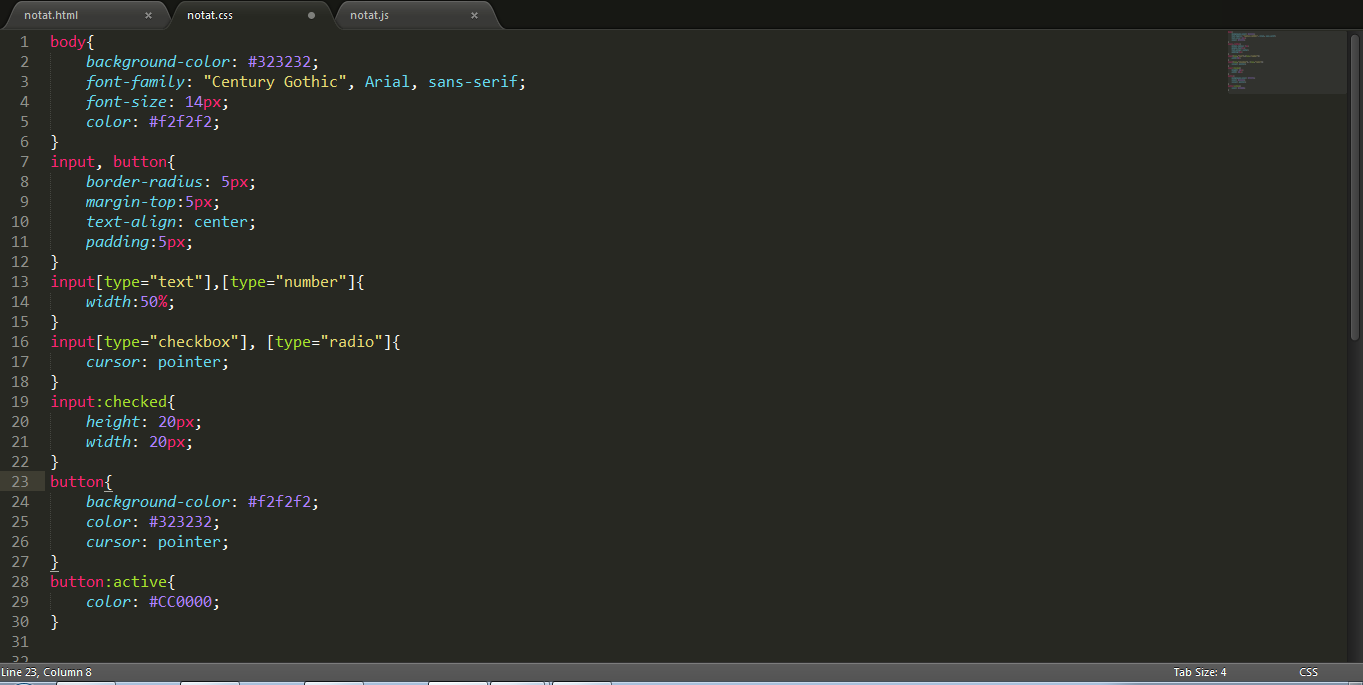
\includegraphics[width=0.75\linewidth]{css1.png}
\end{figure}
\begin{figure}[h!]
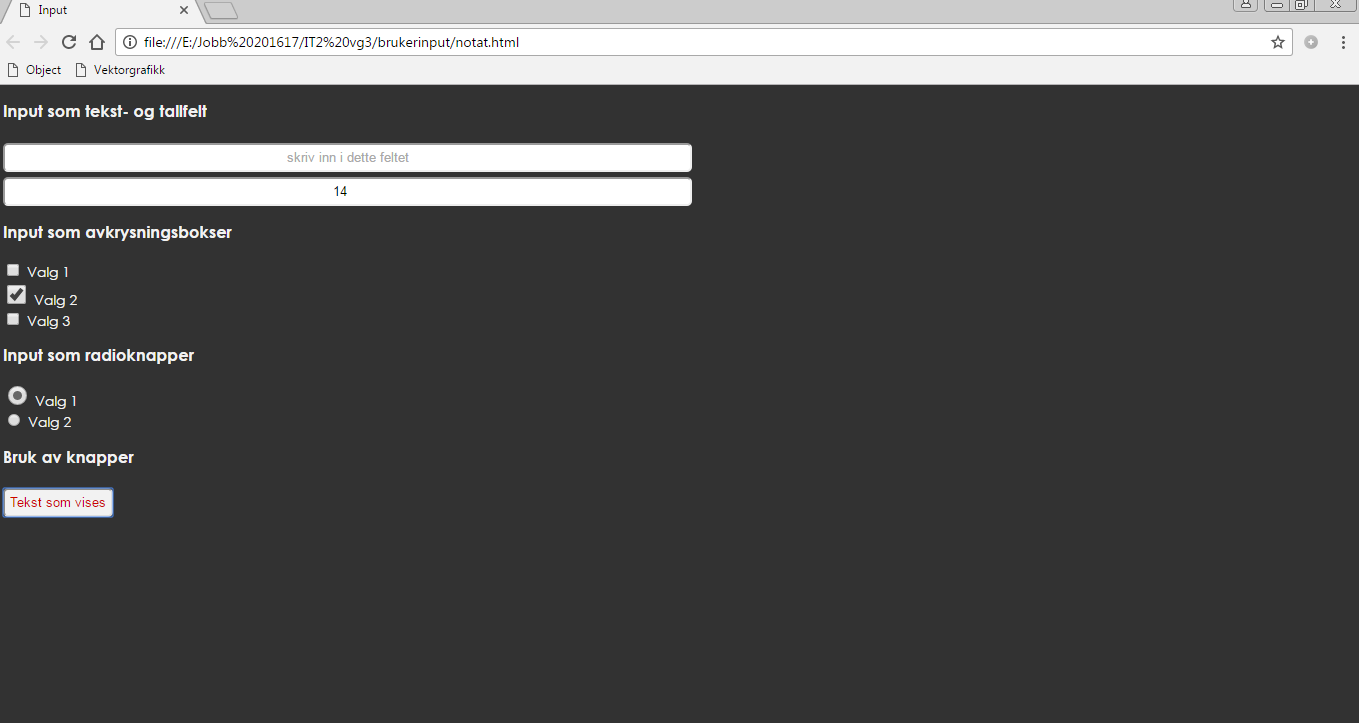
\includegraphics[width=0.75\linewidth]{css2.png}
\end{figure}

\clearpage
\section*{JavaScript}
%\begin{figure}[h!]
%\includegraphics[width=0.5\linewidth]{oppg1a2.jpg}
%\end{figure}
\begin{tabular}{|p{10cm}|p{6cm}|}
\hline
\multicolumn{2}{|c|}{\large{Tekstbokser (text, number) } \cellcolor{lightgray}} \\
var tekstInputEl = document.querySelector("$\#$tekstinput"); & $\bullet$ bruker en hendelsesstyrt funksjon for\\
var tekstInnhold=tekstInputEl.value; &  å lagre innholdet\\
\multicolumn{2}{|c|}{\large{Avkrysningsbokser (checkbox) } \cellcolor{lightgray}} \\
var checkInputEl1 = document.querySelector("$\#$checkinput1"); & $\bullet$ sjekker om boksen er valgt og lar dette\\
if (checkInputEl1.checked)$\{\}$ & styre innholdet i if-setninger\\
& $\bullet$ husk at flere bokser kan velges! \\
\multicolumn{2}{|c|}{\large{Radioknapper (radio) } \cellcolor{lightgray}} \\
var radioInputEl1 = document.querySelector("$\#$radioinput1"); & $\bullet$ sjekker om boksen er valgt og lar dette\\
if (radioInputEl1.checked)$\{\}$ & styre innholdet i if-setninger\\
& $\bullet$ husk at kun en kan velges! \\
\multicolumn{2}{|c|}{\large{Knapper (button)} \cellcolor{lightgray}} \\
var knappEl = document.querySelector("$\#$knapp"); & $\bullet$ knytter en hendelse til knappen\\
knappEl.addEventListener("click", funksjon); &(klikk, dobbelklikk) og lar denne styre \\
function funksjon(e)$\{\}$ & en funksjon som bearbeider input\\
\hline
\end{tabular}\\
\begin{figure}[h!]
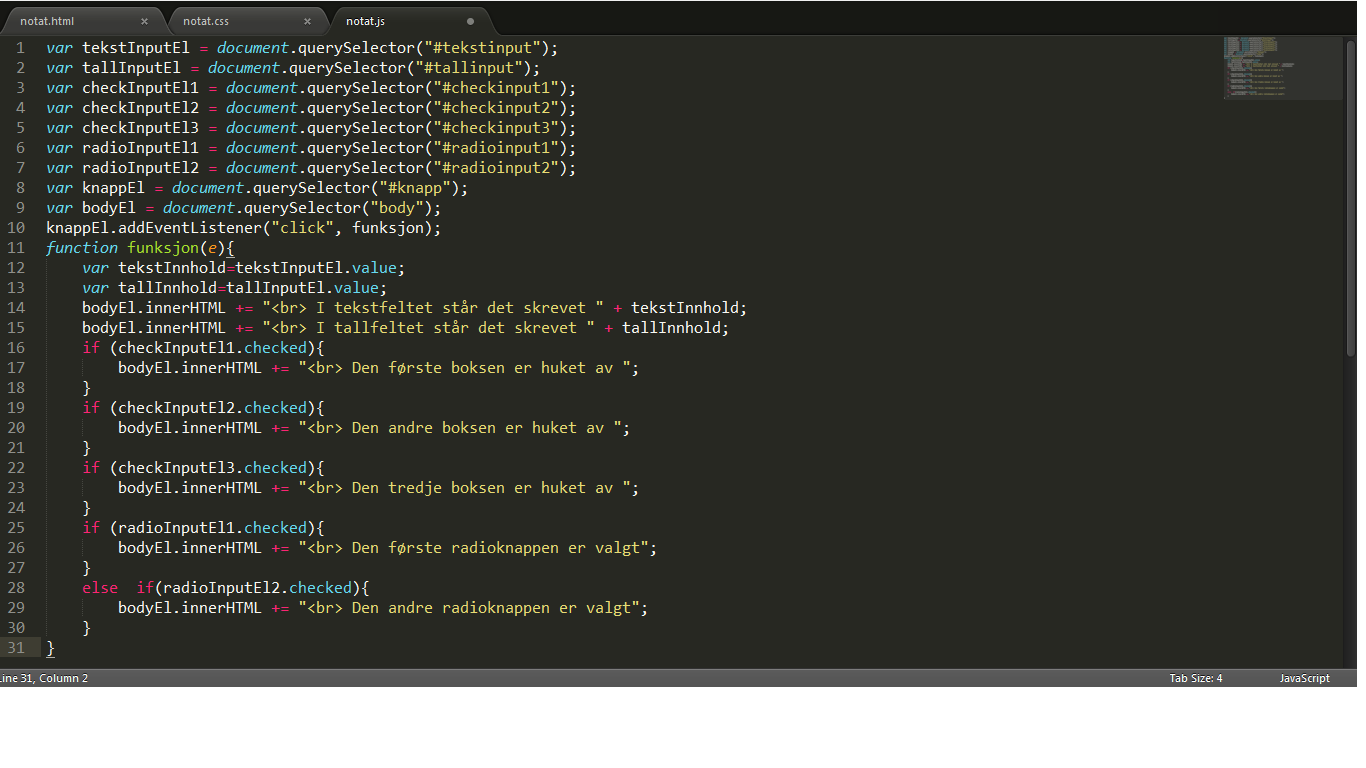
\includegraphics[width=0.8\linewidth]{js1.png}
\end{figure}
\begin{figure}[h!]
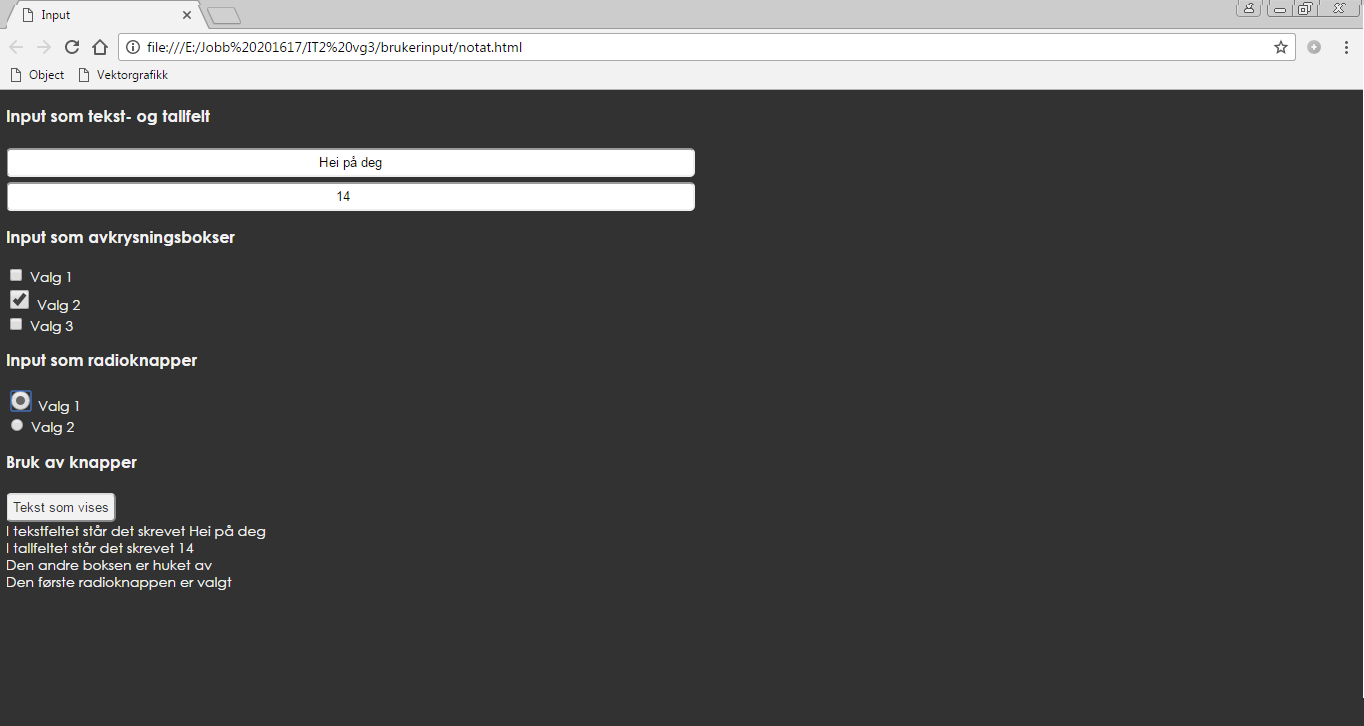
\includegraphics[width=0.8\linewidth]{js2.png}
\end{figure}

\end{document}